\chapter{parelm}

\section{Introduction}

An LPE may have parameters that do not affect the behavior of that process in any way.
These parameters are said to be \emph{inert}.
Removing inert parameters from an LPE reduces the size of state vectors and the state space of that LPE, which both benefits performance.

\section{Algorithm}

The algorithm consists of the following steps \cite{groote2001computer}:

\begin{enumerate}

\item Make it so that all parameters of the LPE are \labeledas{inert}.

\item Consider the guards of all summands of the LPE, and \removelabelfrom{inert} from all LPE parameters that occur in the guard of a summand.

\item Let $X$ be the set of all LPE parameters that are \labeledas{inert}, and consider all expressions $v_s(p)$ that define the value of an LPE parameter $p$ after application of a summand $s$.
For each such expression, if $p$ is \emph{not} \labeledas{inert}, \removelabelfrom{inert} all LPE parameters that occur in $v_s(p)$.

\item Repeat the previous step until the fixpoint of $X$ is reached.
Then remove all LPE parameters that are still \labeledas{inert} from the LPE, substituting references to those parameters by their initial values.

\end{enumerate}

\clearpage
\section{Example}

Consider the following LPE:

\begin{lstlisting}
//Process definition:
PROCDEF example[A :: Int, B](x, y, z :: Int)
  = A ? i [[x==0]] >-> example[A, B](i, y, z)
  + A ? i [[x==1]] >-> example[A, B](0, i, z)
  + B [[x==2]] >-> example[A, B](0, y, z)
  + B [[true]] >-> example[A, B](z, y, x)
  ;

//Initialization:
example[A, B](0, 0, 0);
\end{lstlisting}

First, the `inert' label is removed from $x$ because $x$ occurs in the guards of the first three summands.

In the fourth summand, $z$ is used in the expression of which the value is assigned to $x$.
Therefore $z$ is also no longer \labeledas{inert}.

$y$ remains labeled with `inert': it does not occur in a guard, nor is it used in the assignment to a process parameter other than itself.
Removing $y$ gives

\begin{lstlisting}
//Process definition:
PROCDEF example[A :: Int, B](x, z :: Int)
  = A ? i [[x==0]] >-> example[A, B](i, z)
  + A ? i [[x==1]] >-> example[A, B](0, z)
  + B [[x==2]] >-> example[A, B](0, z)
  + B [[true]] >-> example[A, B](z, x)
  ;

//Initialization:
example[A, B](0, 0);
\end{lstlisting}

\section{Benchmark results}

The following durations were measured with a benchmark for several models:
\begin{itemize}
\item The average duration of \txs{} to make 500 steps in a model after it has been converted to LPE form;
\item The average duration of \txs{} to make 500 steps in a model after it has been converted to LPE form and after the \texttt{parelm} operation has been applied.
\end{itemize}

When plotting the second series of measurements against the first (see Figure~\ref{parelm-vs-lpe-only:fig}), it is easy to see that the impact is insignificant in most cases.
The only model for which a significant performance increase has been measured is the \texttt{ControlLoop} model, which has indeed lost part of its state vector.

\begin{figure}[!ht]
\begin{center}
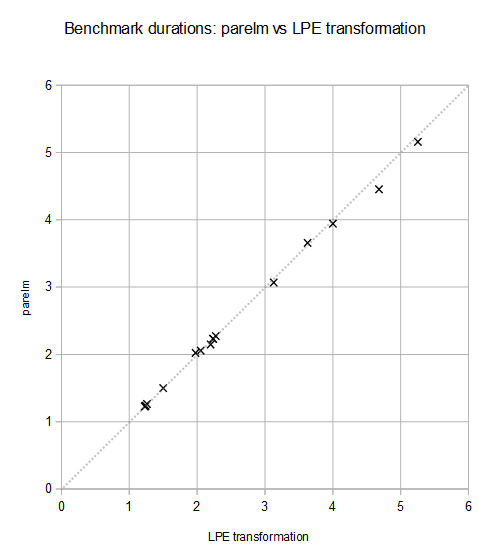
\includegraphics[width=0.5\linewidth]{charts/parelm-vs-lpe-only}
\caption{Benchmark results: parelm vs LPE transformation}
\label{parelm-vs-lpe-only:fig}
\end{center}
\end{figure}

